In this section, first the approaches of the IKC and TM frameworks towards interval representation are compared. Next, their approaches towards the evaluation of Allen relationships between a crisp interval and an interval subject to uncertainty are compared.

\subsection{\label{subsec:comp-interval}Comparison of Approaches to Interval Representation}
The IKC framework uses IKTI to represent time intervals subject to uncertainty, whereas the TM framework uses UTI for this. In both approaches, to consider uncertainty about the exact CTI which is intended, uncertainty about the exact starting and ending instants of the intended interval is considered and confidence in the context of this uncertainty is expressed using two possibility distributions. In an IKTI, these possibility distributions each define one IKV. One of these then defines the IKTI's starting instant and the other defines its ending instant. In an UTI, one of these possibility distributions is directly meant to define the UTI's starting instant and the other is directly meant to define the UTI's ending instant. It is obvious that the concepts of IKTI and UTI are exactly the same, except for the explicit usage of the concept of IKV in IKTI to define and describe uncertainty about starting and ending instants. This equality implies that both approaches have the same basic restriction: they cannot represent every kind of interval subject to uncertainty imaginable. For example, imagine an ordered set of instants coinciding with $\mathbb{N}_0$ and imagine an interval subject to uncertainty in this set, where the intended interval is either $\left[2, 4\right]$ (possibility $1$) or $\left[3, 7\right]$ (possibility $1$). This interval can not be modelled by a combination of possibility distributions defining the starting and ending instants without making $\left[2, 7\right]$ and $\left[3, 4\right]$ also possible as intended intervals to some extent. This issue was first suggested about IKTI in~\cite{Billiet2012}.

Now, a major difference between the two frameworks, concerning their approaches towards the representation of time intervals in general, is that the TM framework includes visualization in its approach.

A first consequence of this is that the TM framework allows the visualization of multiple CTI in the same image plane. In theory, it should also allow the visualization of multiple UTI in the same image plane. However, if the interval space area's visualizing these UTI overlap, it is not yet researched which greyscale (or other) color and intensity each interval point in this overlapping area should have, as the appearance of such interval point should both reflect the possibility of it being the interval intended by the one UTI and the possibility of it being the interval intended by the other UTI. The advantage of the ability to visualize multiple time intervals in the same image plane is that a human observer could easily assess certain characteristics of a distribution of time intervals from an image containing their visualization. The IKC framework, on the other hand, doesn't incorporate any form of visualization and doesn't allow such human assessments.

A second consequence of this is that the TM framework requires that an UTI can be visualized, using a visualization method which actually visualizes the possibility of a CTI of being the interval intended by this UTI for every CTI that has a non-zero possibility of this. Thus, a method is required, to calculate the possibility of a given CTI of being the interval intended by an UTI based on the possibility distributions defining this UTI. This method is found by demanding that the given CTI's starting instant is the intended interval's starting instant \emph{and} that the given CTI's ending instant is the intended interval's ending instant and by determining the possibility of the conjunction of both demands using the standard possibility theory conjunction operator `minimum'. Although not necessary for the correct and consistent functioning of the TM framework, it appears to be the intention of the TM framework that possibility about the exact starting or ending instant of the interval intended by the UTI could be derived from the possibility distribution defining the possibility that a given CTI is the interval intended by the UTI. For this derivation to be consistent, the possibility distributions defining the UTI must be convex~\cite{Dubois1983}. Given an ordered set $T$ and an UTI $J = (\pi_{J_s}, \pi_{J_e})$ in $T$ with possibility $\pi_J(I)$ that a given CTI $I = \left[s_i, e_i\right]$ is the exact time interval intended by $J$, the derivations can be calculated as follows:
\vspace{-5pt}
\begin{align}
\pi_{J_s}(s_i) = \max_{K = \left[s_i, k\right], k \in T, k > s_i}(\pi_J(K)) \nonumber \\
\pi_{J_e}(e_i) = \max_{K = \left[k, e_i\right], k \in T, k < e_i}(\pi_J(K)) \nonumber
\end{align}

With respect to this convexity demand, the IKC framework is similar: the possibility distributions defining the starting and ending IKV of an IKTI are also demanded to be convex by the IKC framework, although this appears not to be necessary for the framework to function correctly and consistently.

\subsection{\label{subsec:comp-eval}Comparison of Approaches to Allen Relationship Evaluation}
As mentioned before, a major difference between the two frameworks, concerning their approaches towards the representation of time intervals in general, is that the TM framework includes visualization in its approach. As a result, it also includes visualization in its approach towards the evaluation of Allen relationships between a CTI and an UTI.

A first consequence of this is that, given a CTI, an UTI, its URZ and their visualizations in the same image, the TM framework allows a visual, human assessment of the degree of possibility of this CTI being in an Allen relationship with this UTI, for every Allen relationship with a non-zero such degree, based on this image. Moreover, those with possibility degree equal to zero can be easily found before any calculation is done: they are the relationships not contained in the set corresponding to the URZ containing the CTI's interval point. On the other hand, to examine the respective possibilities of a given CTI of being in several different Allen relationships with a given IKTI using the IKC framework, a new collection of specific IKC and a specific aggregation of these should be constructed for every Allen relationship under consideration, allowing to calculate its exact possibility and necessity. In contrast to the TM framework, using the IKC framework a human assessment before any calculation is not possible and it is not known before any calculation which Allen relationships will result in a possibility degree equal to zero.

A second consequence is that, given an UTI and its URZ, multiple CTI can be visualized in the same image as the UTI and its URZ. Thus, the same image could provide a visual, human assessment of the possibilities with which multiple CTI are in Allen relationships with the UTI, before any calculation is done. Again, the IKC framework would need a different collection of specific IKC and a specific aggregation of these for every Allen relationship under consideration, but calculating the possibilities for several CTI to be in a given Allen relationship with a given IKTI would not provide much extra work.

A third consequence is that, in the TM framework, given an UTI, its URZ and a visualization of these in the same image, a given Allen relationship could correspond with several URZ. Thus, given a distribution of CTI, it is not easy to visually assess which CTI have a non-zero possibility of being in the given Allen relationship with the given UTI. On the other hand, assessing this using the IKC framework is impossible without any calculation, but the necessary calculations are pretty straightforward.

Although this has not been rigorously researched yet, it is the conviction of the authors that a great strength of the IKC framework lies in its modular approach towards the evaluation of temporal relationships, resulting in a flexibility and an easy handling of complex temporal relationships, while the visualization of these using the TM framework could become complex and heavy. This would give the IKC framework a major advantage over the TM framework, when used in reasoning systems like e.g. decision support systems. Moreover, in some cases the visualization step used in the TM framework could be a redundant step.

\subsection{\label{subsec:example}An Example}
In this section, some of the comparison results presented above will be illustrated using a simple example.

\begin{example}
Consider an ordered set of instants $T$ coinciding with $\mathbb{R}$, a CTI $I = \left[1, 3\right]$ and a time interval $J$ of which the starting instant is defined by a triangular possibility distribution on $T$ with core $\{5\}$ and support $\left[2, 7\right]$ and of which the ending instant is defined by a triangular possibility distribution on $T$ with core $\{12\}$ and support $\left[9, 15\right]$. In a real-life situation, such distributions could be decided by experts or deduced from existing evidence. The visualization of this example situation using the TM framework is shown in figure \ref{fig:ex}. The interval point for $I$ lies in the URZ `PM'. Thus, possibility is higher than zero for $I$ to be in a `meets', `before', or `overlaps' relationship with $J$. As the darkest point in the `overlaps' area part is very light, the darkest point in the `meets' line segment is of almost exactly the same lightness and the darkest point in the `before' area part is perfectly black, it can be estimated that $I$ overlaps $J$ with a low possibility, $I$ meets $J$ with the same low possibility and $I$ is before $J$ with possibility $1$. Calculation using the IKC framework now learns that:
\vspace{-5pt}
\begin{align}
\Pos(I overlaps J) & = \min(1, 1/3, 1) = 1/3 \nonumber \\
\Pos(I meets J) & = \min(1, 1/3) = 1/3\nonumber \\
\Pos(I before J) & = \min(1) = 1\nonumber
\end{align}
\end{example}
\vspace{-10pt}

\begin{figure}[h]
	\centering
	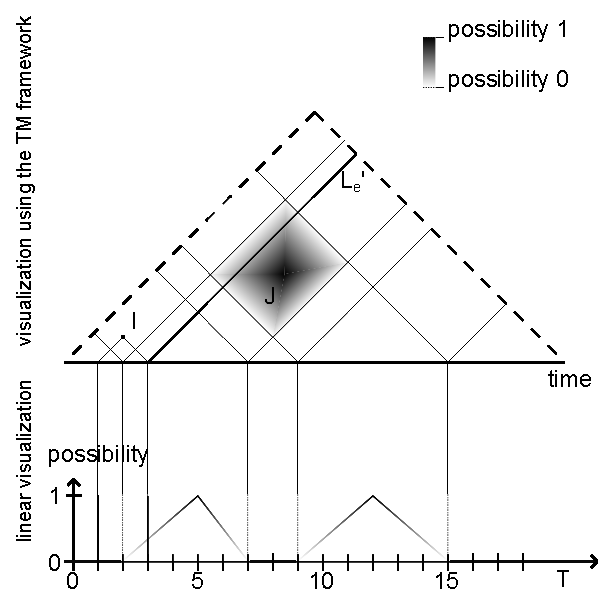
\includegraphics[width=0.9\columnwidth]{graphs/example_image.eps}
	\caption{The visualization of the example using the TM framework.}
	\label{fig:ex}
\end{figure}
\vspace{-5pt}